\documentclass{beamer}
\usepackage{listings}
\begin{document}
\title{Python Chapter 1}
\author{Ezequiel Torres}
\date{\today}
\frame{\titlepage}
\frame{\frametitle{Table of contents}\tableofcontents}

\section{Before getting started}
\frame{\frametitle{Before getting started}
    We will be going over the basics of python and interviewing in python in this course.
    Here are some great resources to get started.
    \begin{itemize}
        \item<1-> http://programarcadegames.com
            \begin{itemize}
                \item<2-> Fun way to learn python at your own pace while making arcade games!
            \end{itemize}
        \item<3-> https://www.crackingthecodinginterview.com/
            \begin{itemize}
                \item<4-> 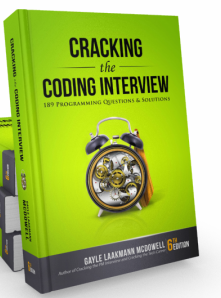
\includegraphics{CTCI.png}
            \end{itemize}
    \end{itemize}
}
\frame{\frametitle{Before getting started}
    \begin{itemize}
        \item<1-> https://www.amazon.com/Grokking-Algorithms-illustrated-programmers-curious/dp/1617292230
            \begin{itemize} 
                \item<2-> 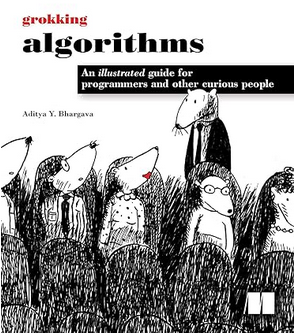
\includegraphics{ga.png}
            \end{itemize}
        \item<3-> https://github.com/zeaktorres/WSU-Python-Workshop-2024/
            \begin{itemize}
                \item<4-> Where the notes will be stored 
            \end{itemize}
    \end{itemize}
}

\section{Basic Expectations}
\frame{\frametitle{Basic Expectations}
    There are a few things this course considers you have a basic understanding of.
    \begin{enumerate}
        \item<1-> The terminal
        \item<1-> Basic programming in C or C++
        \item<1-> Some understanding of data structes (however we will cover this too)
    \end{enumerate}
    It is perfectly fine if you do not feel like an expert in any of these fields, please feel free to raise you hand if you 
    have any questions about any of these.
}


\section{Environment setup}
\frame{\frametitle{Environment setup}
    Here are the basic steps to running python. 
    \vspace{\baselineskip}

    On a Windows PC, you will download the exe: https://www.python.org/downloads/. 
    \vspace{\baselineskip}

    On Linux, use the appropriate package manager. The schools Linux lab uses X so you will use "sudo ....", however they should have python already installed.
    \vspace{\baselineskip}

    On Mac, idk. If you have a Mac and are having trouble running python let me know, I will be able to help you
}

\frame{\frametitle{IDE?}
    Well this is the more... unique part? Essentially you can choose whatever editor you want. You don't even have to use an IDE, you can edit python in 
    notepad++! Then, when you want to run the SCRIPT, simply run "python SCRIPT" in the terminal.

    \begin{enumerate}
        \item<1-> Python's own IDE, yeah probably don't use this one
        \item<1-> VSCode, a very popular text editor in electron. Great for industry practice
        \item<1-> Pycharm, I don't have much experience with pycharm but I've heard great things if you want to give it a shot
        \item<1-> Neovim/Vim, I personally use Neovim because I hate myself
    \end{enumerate}

}

\section{Variables}
\frame{\frametitle{Variables} 
    Here we will go into some basic examples of variables in python.
    First, variables should be lowercase
    \vspace{\baselineskip}

    Also, variables are not typed like in C or C++ since python is a dynamically typed language. Meaning the variables
    are determined at runtime

    \begin{enumerate}
        \item<1-> x = 5
        \item<1-> y = 10
        \item<1-> print(x + y)
    \end{enumerate}
    15
}
\subsection{Variables and Concatenation}
\frame{\frametitle{Variables and Concatenation} 
    "In formal language theory and computer programming, string concatenation is the operation of joining character strings end-to-end" - Wikipedia 
    \vspace{\baselineskip}

    IE: print("Hello" + "World")
}
\subsection{Variables Exercise}
\frame{\frametitle{Variables Exercise}
    Write a python program which prints a users mpg. You can take in input in python like the following:
    \vspace{\baselineskip}

    miles\_driven = input("Enter the number of gallons")
    \vspace{\baselineskip}

    Note: These exercises are purposely vague as are interview questions to get you to ask important questions
    \vspace{\baselineskip}

    Note: Sometimes interviewers will give you hints if you are struggling but some interviewers will take taking a hint as a negative
}

\section{Operators and If Statements}
\subsection{Operators}
\frame{\frametitle{Operands}
    Here we will get into the basic applications of operands in python.
\begin{tabular}{|l||l||r|}
\hline
    operator & operation & example \\ 
\hline
    + & addition & a = 3 + 2\\ 
\hline
    - & subtraction & a = 3 - 2\\
\hline
    * & multiplication & a = 3 * 2\\
\hline
    / & division & a = 10 / 2\\
\hline
    \% & modulus & a = 8 \% 3 (remainder of 8 / 3 is 2)\\
\hline
\end{tabular}
}

\subsection{If statement}
\begin{frame}[fragile]
\frametitle{If Statement example}
  \begin{lstlisting}
       x = 5
       y = 6

       if x > y:
        print("x is greater than y")
       else:
        print("y is greater than or equal to x")
   \end{lstlisting}
\end{frame}


\subsection{Operators and If Statements Exercise}
\frame{\frametitle{Operators and If Statements Exercise}
    Fizz Buzz Simple: Take in an integer n, return Fizz if the number is even, and Buzz if the number is odd 
}


\end{document}
